


\subsection{Architecture}
For the implementation of the client application, \textit{React.js} which aims to solve the challenges involved when developing web application with complex user interfaces, is applied. To have a better concept of how Graphicuss's client application is implemented, an overview of the file structure is listed in the figure \ref{fig:server-file-structure-imp}.

\subsubsection{Project Structure}
\begin{figure}[!htbp]
\centering
\begin{forest}
  for tree={
    font=\ttfamily,
    grow'=0,
    child anchor=west,
    parent anchor=south,
    anchor=west,
    calign=first,
    edge path={
      \noexpand\path [draw, \forestoption{edge}]
      (!u.south west) +(7.5pt,0) |- node[fill,inner sep=1.25pt] {} (.child anchor)\forestoption{edge label};
    },
    before typesetting nodes={
      if n=1
        {insert before={[,phantom]}}
        {}
    },
    fit=band,
    before computing xy={l=15pt},
  }
[client
  [components/
    [AppBar/
      [index.js]
      [style.css]
    ]
    [...]
  ]
  [containers/]
  [models/]
  [utils/]
  [index.js]
  [index.html]
  [...]
]
\end{forest}
\caption{Overview of server app's file structure}
\label{fig:server-file-structure-imp}
\end{figure}

\begin{itemize}
  \item 
  \textbf{components/}: all components are defined by extending basic \textit{React.Compoent}. Each custom component has an \textit{index.js}, which processes the logics of view rendering and applies view model to the template. \textit{style.css} defines the CSS style of the HTML DOMs within a component.
  \item 
  \textbf{containers/}: containers are compositions of components.
  \item 
  \textbf{models/}: in model directory, data models for the components are defined. In addition, the definition of APIs and processing after data acquisition  also take place here.
  \item 
  \textbf{index.js \& index.html}: \textit{index.js} is the entry point of the app, which will instantiate the React instance and render the views into a specific DOM defined  in \textit{index.html}
\end{itemize}


\subsubsection{Achitecture of Client}

An overview of the client application's architecture is revealed in figure \ref{fig:client-arch-imp}. 

\begin{figure}[!htbp]
  \centering
    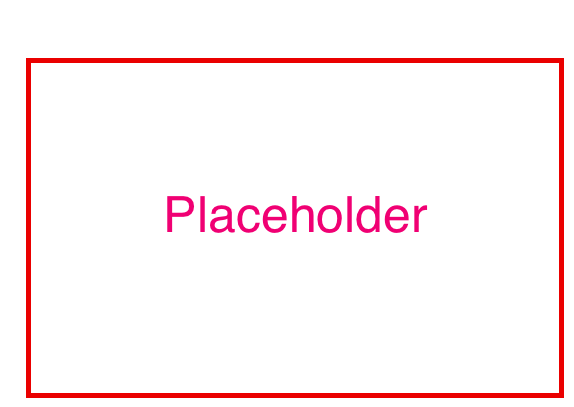
\includegraphics[width=0.6\textwidth]{Figures/placeholder.png}
  \caption{Overview of client architecture}
  \label{fig:client-arch-imp}
\end{figure}
% client arch, App -> router containes rotes -> different container -> components(Compisition... for containers!)

In the React application, \textit{Router} is also regarded  as a component, in which different matching rules of URL are defined. If the URL requested by user is matched, a correlate view will be rendered according to the definition of routes. Code list \ref{list:router-client-imp} shows the implementation of defining a \textit{Router} component.

\begin{lstlisting}[language=HTML, caption=Router in client app , label={list:router-client-imp}]
<Router history={history}>
  <Route path="/" component={App}>
    <Route path="auth" component={AuthView} />
    <Route path="courses" component={CoursesView} />
    <Route path="courses/:courseId" component={QuestionsView} />
    <Route path="questions/:questionId" component={AnswersView} />
  </Route>
</Router>
\end{lstlisting}








\subsection{Composition of Components}

\subsubsection{React Component}


\subsubsection{Composition}
\textit{Components} are the core of React. All each view and its view model of the client application is represented as a React \text{Component}. And the whole client app is actually a composition of React components. An example of \textit{CoursesView} is taken in figure \ref{fig:course-view-composition-imp}.

\begin{figure}[!htbp]
  \centering
    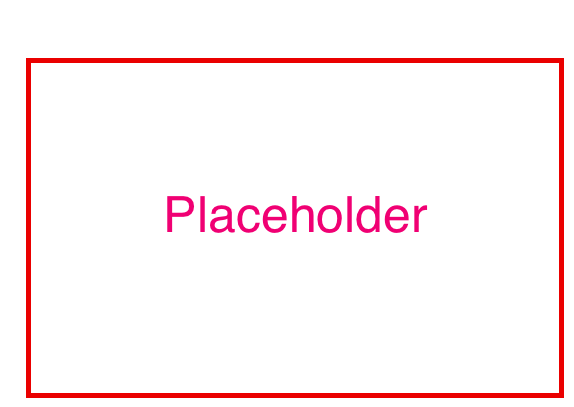
\includegraphics[width=0.6\textwidth]{Figures/placeholder.png}
  \caption{Composition of components in courses' page}
  \label{fig:course-view-composition-imp}
\end{figure}
% Course Page. Composition, App bar, tab view, course page, course card ...

At the top of the view is a component called \textit{AppBar}, which is also composed with another component \textit{SearchBox}. \textit{ContentSection} is a container for the main content, which will be replaced and re-rendered if the context of router changes. In this example, the route \textit{/courses} is applied, and the component \textit{CourseView} is rendered into \textit{ContentSection}. 

\textit{CourseView} is also a composition of components: a list of \textit{CourseCard} components and also other components such as submit button component and popover component for creating new course. 

In principle, building other views is the same approach. Composition of components constructs the all views. With fine-grained components, the client app becomes much extensible and maintainable.


\subsection{Data Flow}

\subsubsection{Flux Architecture}

\subsubsection{Data Fetching}
